%%%%%%%%%%%%%%%%%%%%%%%%%%%%%%%%%%%%%%%%%%%%%%%%%%%%%%%%%%
%% Task 3
%%%%%%%%%%%%%%%%%%%%%%%%%%%%%%%%%%%%%%%%%%%%%%%%%%%%%%%%%%

Given a model with couples already created, Task 3 consists in calculating the average rating of shared movies for each of these couples. As for the previous tasks, we provide solutions both in e-Motions and Maude. 

%%%%%%%%%%%%%%%%%%%%%%%%%%%%%%%%%%%%%%%%%%%%%%%%%%%%%%%%%%%%%%%
\subsubsection{e-Motions-based solution.}

The solution consists in one single rule, shown in Figure~\ref{fig:computingAvgRating}, in which the average is calculated only once for each couple. Notice the use of an action in the NAC of the rule to state that the value has not been already calculated. The number of rewrites and execution times for $N=2, 10$ are shown in Table~\ref{table:emotionstask3}.

\begin{figure}[htp]
  \centering
  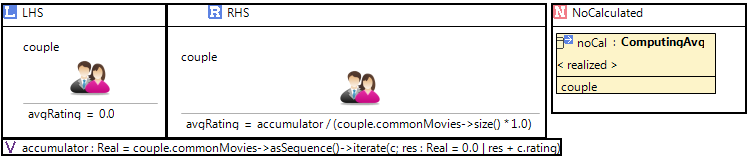
\includegraphics[width=\textwidth]{imgs/computingAvgRating}
  \caption{\code{computingAvgRating} rule.}\label{fig:computingAvgRating}
\end{figure}

\begin{table*}[tb]
\renewcommand{\tabcolsep}{6pt}
\renewcommand{\arraystretch}{1.2}
    \centering
	\begin{tabular}{r r r}
	$N$ & Time (s) & \# Rewrites \\
	\hline
	2 & 0.0 & 4,527 \\
	10 & 2.1 & 891,432 \\
	\hline \\
	\end{tabular}
	\caption{e-Motions times for Task 3.}\label{table:emotionstask3}
\end{table*}

%%%%%%%%%%%%%%%%%%%%%%%%%%%%%%%%%%%%%%%%%%%%%%%%%%%%%%%%%%%%%%%
\subsubsection{Maude-based solution.}
The corresponding Maude rule specifying the solution of this task is shown in Listing~\ref{lst:task3}. Table~\ref{} show the number of rewrites and execution times for problems of sizes $100$, $200$, $300$, and $400$.

\begin{lstlisting}[caption=Maude rule for Task 3 solution., label=lst:task3]
crl [avgRating] :
  { < M : Couple | commonMovies : MovieSet, 
       avgRating : 0.0, 
       Atts1 >
    couplesCalculated(Couples) 
    C 
  }
=>
  { < M : Couple | commonMovies : MovieSet, 
       avgRating : sumAllRatings(MovieSet, C) 
                     / float(| MovieSet |),
       Atts1 >
    couplesCalculated((M, Couples)) 
    C
  }
if not(M in Couples) .
\end{lstlisting}

\begin{table}
  \begin{center}
	\begin{tabular}{r r r}
	$N$ & Time (s) & \# Rewrites \\
	\hline
	100 & 1.5 & 21,800 \\
	200 & 6.3 & 43,600 \\
	300 & 14.9 & 65,400 \\
	400 & 29.7 & 87,200 \\
	\hline \\
	\end{tabular}
	\caption{Maude times for Task 3.}\label{table:maudetask3}
	\end{center}
\end{table}